\documentclass[12pt,a4paper]{article}

\usepackage{natbib}
\usepackage{graphicx}
\usepackage{hyperref}
\usepackage[page,toc,titletoc,title]{appendix}
\usepackage{listings}
\usepackage{color}
\usepackage[nottoc,notlof,notlot]{tocbibind}
\usepackage{amsfonts}
\usepackage[skip=10pt]{parskip}
\usepackage{float}

\definecolor{keyword}{rgb}{0,0,0.5}
\definecolor{number}{rgb}{0, 0, 1}
\definecolor{string}{rgb}{0, 0.5, 0}
\definecolor{comment}{rgb}{0.5, 0.5, 0}
\definecolor{grey}{rgb}{0.5, 0.5, 0.5}
\graphicspath{ {./img/} }
\lstset{
    language=Python,
    basicstyle=\footnotesize\ttfamily,
    commentstyle=\color{comment},
    keywordstyle=\color{keyword},
    numberstyle=\color{number},
    stringstyle=\color{string},
    breaklines=true,
    frame=single,
    numbers=left,
    numbersep=5pt,
    numberstyle=\tiny\color{grey},
    showspaces=false,
    showstringspaces=false
}

\begin{document}
    \title{chizuru-rogue: Deep Learning for Dungeon Crawling}
    \author{Dylan G. Drescher\\[1ex]Supervisor: Dr. Jie Zhang\\[1ex]B.Sc. Computer Science - University of Bath}
    \date{2022 - 2023}
    \maketitle

    \setcounter{page}{0}
    \thispagestyle{empty}

    \newpage
    \pagenumbering{roman}

    \begin{center}
        \section*{Declaration of Access}

        This Dissertation may be made available for consultation within the University Library and may be photocopied or lent to other libraries for the purposes of consultation.
    \end{center}

    \newpage

    \textbf{CHIZURU-ROGUE}

    submitted by Dylan G. Drescher

    \section*{Copyright}
    Attention is drawn to the fact that copyright of this dissertation rests with its author.
    The Intellectual Property Rights of the products produced as part of the project belong to the author unless otherwise specified below, in accordance with the University of Bath's policy on intellectual property (see \href{https://www.bath.ac.uk/publications/university-ordinances/attachments/Ordinances_1_October_2020.pdf}{here}).
    This copy of the dissertation has been supplied on condition that anyone who consults it is understood to recognise that its copyright rests with its author and that no quotation from the dissertation and no information derived from it may be published without the prior written consent of the author.

    \section*{Declaration}
    This dissertation is submitted to the University of Bath in accordance with the requirements of the degree of Bachelor of Science in the Department of Computer Science.
    No portion of the work in this dissertation has been submitted in support of an application for any other degree or qualification of this or any other university or institution of learning.
    Except where specifically acknowledged, it is the work of the author.

    \newpage

    \addcontentsline{toc}{subsection}{Abstract}
    \begin{abstract}
        \noindent Video games are one of the most popular problem domains to tackle with reinforcement learning due to the interesting complexity that can arise from simple sets of rules that many games provide.
        By training reinforcement learning models on video games and proving they are effective at solving problems, they can then be repurposed for other problems such as self-driving cars to make decisions about speed and navigation,
        and healthcare to optimise and personalise treatment plans.

        \noindent In this article we introduce chizuru-rogue, which is a computer program designed to play Rogue, a well-known dungeon-crawling game regarded as the pioneer of the ``roguelike'' video game genre, which is characterised by randomly generated levels, turn-based gameplay and permanent character death.
        Rogue offers a unique problem to solve, requiring a player to solve partially observable, randomly generated levels.

        \noindent chizuru-rouge interfaces with a program called Rogue-gym, a program that accurately mimics the gameplay of Rogue and
        the agent utilises a Rainbow Deep Q-network to explore the dungeon, collect gold and reach the goal of collecting the Amulet of Yendor. % customised neural network that involves an LSTM for long-term and short-term memory to explore levels in Rogue

        \noindent TensorFlow will be used as a framework to implement the reinforcement learning agent.
        TensorFlow is a Python library that provides tools to streamline development of deep learning models.
    \end{abstract}

    {\footnotesize \textbf{Keywords - reinforcement learning, neural networks, deep q-learning, roguelikes, video games, machine learning}}

    \newpage

    \addcontentsline{toc}{subsection}{Acknowledgements}
    \begin{center}
        \section*{Acknowledgements}
        I would like to express my gratitude to my supervisor Dr. Jie Zhang for providing me with invaluable guidance
        and feedback on my dissertation throughout the year, my parents for their proofreading and the administrators
        of Hex, the university GPU cloud for providing me with computational power to run my model on.
    \end{center}

    \newpage

    \tableofcontents
    \listoffigures
    % \listoftables

    \newpage

    \pagenumbering{arabic}

    \section{Introduction}\label{sec:introduction}
    Rogue is a 1980 computer game that belongs to a genre called ``roguelikes''.
    Roguelikes are characterised by challenging, turn based dungeon crawling gameplay, procedurally generated levels and permanent character death.
    They are inspired by Rogue.
    This genre of game offers a fascinating domain to apply reinforcement learning methods to due to the amount of strategies and gameplay styles that roguelike games allow.
    In these games, turns often resolve immediately, allowing for efficient training.

    The aim of chizuru-rogue is to apply deep reinforcement learning methods for an agent to learn and survive within Rogue.
    Reinforcement learning works by an agent using the current state to decide on an action to do, then observing a reward for that action, as well as a resulting new state.
    Reinforcement learning is suitable for this problem domain because games provide rewards for skilled play, allowing for training.
    The hope is chizuru-rogue will be able to play the game to a level where it can reach the Amulet of Yendor, the goal of the game.

    Should the project prove successful, it can serve as a foundation for creating AI to play more complex
    roguelike games like NetHack\footnote{\url{https://nethackwiki.com/wiki/NetHack}}.

    \subsection{Rogue - the game}\label{subsec:rogue}
    \subsubsection{Objective}\label{subsubsec:objective}
    In Rogue, the player's main objective is to get a high score by descending the Dungeon of Doom to slay monsters, collect gold coins, retrieve the Amulet of Yendor and escape the dungeon with it alive.
    The game is turn based, which means the player can spend as long as they want thinking their next move before the game processes the environment.
    Figure~\ref{fig:rogsc} depicts an example screenshot of the game.

    \begin{figure}[ht]
        \caption[A screenshot of an example Rogue game.]{A screenshot of an example Rogue game. The player is represented with \texttt{@}, stairs with \texttt{\%}, a kestrel enemy with \texttt{K} and gold with \texttt{*}.}
        \centering
        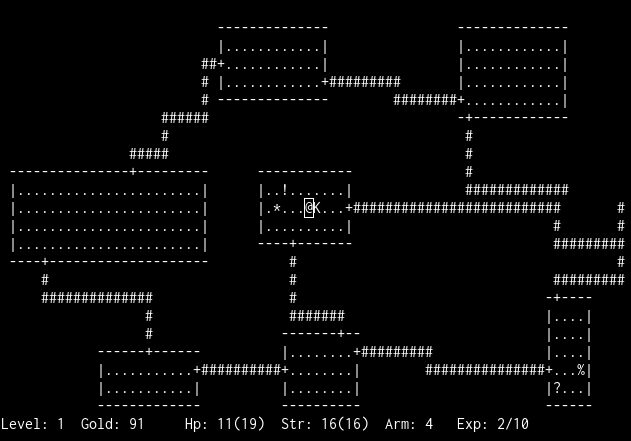
\includegraphics[scale=0.5]{rogue_screenshot}
        \label{fig:rogsc}
    \end{figure}

    \subsubsection{Environment}\label{subsubsec:environment}
    The dungeon's floors are randomly generated mazes made up of several rooms connected with corridors.
    Rooms may be empty or populated with several items or enemies, and one will have stairs to descend to the next floor,
    represented with the character \texttt{\%}.
    When the player starts a new run\footnote{A play-through of the game from start to finish.}, the player is placed in dungeon level 1 with basic equipment.

    Rogue's environment is partially observable;
    the dungeon configuration is initially obscured to the player, revealing itself as the player moves around.

    The game tracks several stats that are always shown to the player:
    \begin{itemize}
        \item \textbf{Level} denotes the current dungeon level.
        \item \textbf{HP} (Hit Points) represents how much damage the player can take before death.
        The number in brackets is the player's maximum HP.
        \item \textbf{Str} (Strength) represents how strong the player is.
        The number in brackets is the player's maximum strength.
        \item \textbf{Gold} is how many gold coins the player has collected.
        Gold increases the player's final score.
        \item \textbf{Arm} (Armour) is the player's current armour rating.
        The higher the rating, the higher chance to avoid attacks.
        \item \textbf{Exp} shows the player's experience level and total experience points.
        When the player earns enough experience points, the player's experience level increases, increasing the player's maximum HP.
    \end{itemize}

    \subsubsection{Items}\label{subsubsec:items}
    There are a wide variety of items the player can use, such as potions, scrolls, weapons and armour.
    Some items need to be identified before the player knows what it will do.
    This can either be done by using a scroll of identify, or by blindly using or wearing the item, which may be risky as some items can have negative effects.

    \subsubsection{Combat}\label{subsubsec:combat}
    As the player navigates around the dungeon, they will encounter enemies of increasing difficulty.
    The player can attack enemies by moving into them, attacking them with the equipped weapon.
    Enemies in the game will try to harm the player by attacking and reducing the player's HP\@.
    If the player's HP falls to 0, the player dies and the game ends.

    Unlike many other role-playing games of the time, Rogue uses character permanent death as a mechanic, providing the player with
    the unique challenge of surviving till the end, as the player could not load a previous save if they are defeated.
    Therefore, the player has to think through their future moves much more rigorously;
    the player's decisions have much more weight to them as a wrong move could mean game over.
    \emph{Michael Toy}, Rogue's co-creator, touched on the topic of permanent death in Roguelike Celebration 2016~\citep{gamasutra16} by saying `We were trying to make it more immersive by making things matter \ldots'.

    \subsection{Project Objectives}\label{subsec:objectives}
    The primary objectives of this project are as follows:
    \begin{itemize}
        \item Create a program that uses artificial intelligence to play Rogue.
        This will involve designing, developing and deploying the program to a GPU cloud for training an agent.
        \item Improve upon existing work for playing Rogue.
        As we will explain in Section~\ref{subsec:exploring-rogue}, existing literature has only applied the standard
        DQN\footnote{Deep Q-network: using neural networks to approximate Q-learning.} to Rogue.
        We will investigate into improvements of the DQN algorithm and apply them to play Rogue.
        \item Experiment by using a Dueling DQN, then a Rainbow DQN, both improvements to the original DQN algorithm.
        We will conduct two experiments for this product - training the agent with a Dueling DQN and a Rainbow DQN.
        We will analyse and compare the results of the two experiments.
    \end{itemize}

    \subsection{Summary}\label{subsec:summary1}
    In this section we have introduced our problem domain Rogue, a dungeon crawling game that we will make our program explore.
    Beyond this section, Section~\ref{sec:literature-technology-and-data-review} is focused on the literature review of
    this project, collating and demonstrating previous work on the subjects that are covered on this project.
    Section~\ref{sec:design-and-methodology} will explain in detail the methodology we will use and how we will collect
    results from the upcoming experiments.
    Section~\ref{sec:agent-training-and-results} will focus on discussing the results of the experiments.

    \section{Literature, Technology and Data Review}\label{sec:literature-technology-and-data-review}

    \subsection{Fundamentals of RL}\label{subsec:fundamentals}
    The fundamentals of reinforcement learning and many fundamental algorithms for solving sequential decision problems is explained in detail by~\citet{sutton18}.
    The core idea behind reinforcement learning algorithms is that an agent performs \emph{actions} on an \emph{environment} by deriving what it should do from its \emph{policy}, which is a mapping from states to actions.
    This loop is visualised in Figure~\ref{fig:rlgraph}.
    Once the agent performs an action, it receives the new game state as well as a \emph{reward} signal, telling the agent how good its choice was.

    \begin{figure}[ht]
        \caption[The reinforcement learning loop.]{The reinforcement learning loop. An agent is provided with a state, performs an action and is provided with a reward signal and the resulting state. Image credit: \citet{bhattrl}}
        \centering
        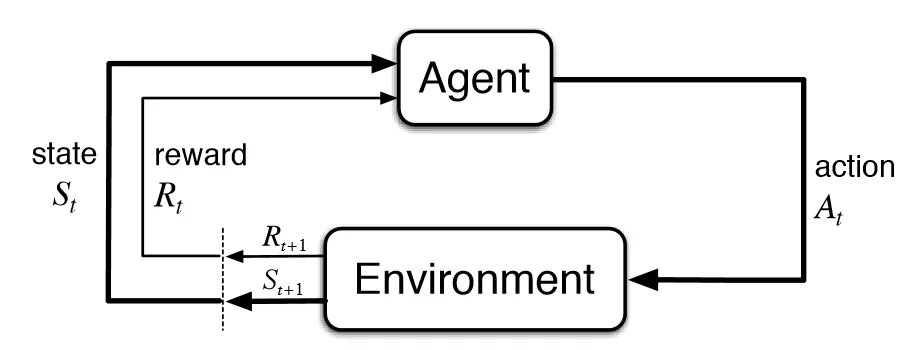
\includegraphics[scale=0.4]{rlgraph}
        \label{fig:rlgraph}
    \end{figure}

    The purpose of rewards is for the agent to constantly estimate a \emph{value function}.
    This function tells the agent either how profitable being in a certain state and following its policy is, or how profitable taking a certain action then following its policy is.
    The theory is that the agent should aim to maximise its cumulative reward by tuning its policy in order to achieve this.

    \subsubsection{Q-learning}
    One of the most well-known reinforcement learning algorithms is the Q-learning algorithm~\citep[chap.~6.5]{sutton18}.
    In this algorithm, the agent keeps track of a table, mapping state-action pairs to its value.
    When the agent reaches a certain state, it consults its Q-table to determine the most valuable action to take.

    The goal of Q-learning is to find the optimal Q-function, which is defined by the Bellman equation:
    \[Q^{*}(s, a) = \mathbb{E} [r + \gamma max_{a'} Q^{*}(s', a')]\]

    This means the optimal value of taking action \(a\) in state \(s\) is the expected reward of taking the action and then following the policy from there.

    \subsection{Deep Learning}\label{subsec:deep-learning}
    Deep learning is a method of artificial intelligence that involves the use of deep neural networks to process data in a way inspired by the human brain.
    This method can also be used in the field of reinforcement learning in order to approximate existing reinforcement learning methods.

    Representing Q-values containing every state-action pairing becomes infeasible in large state spaces such as video
    games, requiring ever expanding tables and computational space needed to store them.
    Deep Q-learning, a technique by OpenAI~\citep{mnih15}, remedies this by using a convolutional neural network to
    approximate the optimal Q-function \(Q^*(s, a)\) using a convolutional neural network instead of keeping track of
    a table.

    The Deep Q-network in their writing was shown to play several Atari games to a superhuman level, most notably Video Pinball and Boxing.
    A similar algorithm involving neural networks was employed by~\citet{silver16} in their development of the AlphaGo system, an agent that was found to beat human grandmaster players in the game of Go.
    The authors used a convolutional neural network alongside ``policy gradient'' reinforcement learning, which is where gradient descent is used to derive a policy.

    While the DQN algorithm by itself is serviceable for simpler problem domains such as Atari, there have been improvements to tackle more challenging domains.
    One of the first improvements to the DQN algorithm is the Double DQN~\citep{hasselt15}, which improves on the original DQN by using a current network for selecting actions
    and then training a ``target network'' to calculate the target Q-value of said action.
    This improves on the original DQN by solving an issue the original DQN had that the Double DQN paper explains in detail,
    where the original DQN suffered from ``substantial overestimations'' when playing Atari games, leading to poorer derived policies due to the fact that
    DQN (and standard Q-learning) uses the save max value for selecting and evaluating an action.
    Using a target network decouples selection from evaluation, according to the paper.

    This is further improved with the Dueling DQN~\citep{wang16}.
    Dueling DQN works by splitting the existing DQN network into two streams: a state-value stream and an ``advantage'' stream.
    Advantage is a value describing how advantageous taking a given action would be given a state-value.
    These streams are then joined with an aggregation layer.
    This saves on computation time due to the intuition that it is not necessary to estimate action-values for each action.

    And finally, Rainbow DQN~\citep{hessel17}, which combines six different techniques to improve upon the Deep Q-network algorithm.
    These techniques are Double DQN, Dueling DQN, Prioritised Experience Replay,
    Multi-step Learning, Distributional RL and Noisy Networks.

    Prioritised Experience Replay~\citep{schaul16} is a technique where experiences in the replay buffer are prioritised in terms of importance and how valuable experiences are to training.
    This way, experiences with higher priority are sampled more often when training happens, allowing for the agent to learn more efficiently.
    Priorities of experiences are adjusted over time so that the agent does not overfit with certain experiences.

    Multistep Learning~\citep[chap.~7.1]{sutton18} is a technique in reinforcement learning that uses sequences of actions and rewards rather than just an individual transition for learning.
    This is in contrast to traditional Q-learning which only takes into account an individual transition for training and calculating action values (a Markov Decision Process framework).
    In multistep learning

    Distributional reinforcement learning~\citep{bellemare17} differs from traditional RL by evaluating a distribution of a random return, rather than a single value for expected returns.
    The goal is to estimate the probability distribution of an expected reward.

    In standard neural networks, weights are deterministic, which means that a certain input will produce only one output.
    Noisy Networks~\citep{fortunato19} introduces a small amount of Gaussian noise within the weights.
    This is because deterministic networks can make the agent get stuck in a suboptimal policy.
    Adding noise to a network can encourage the agent to explore in an efficient manner.
    According to the paper, the key insight is `a single change to the weight vector can induce a consistent and potentially very complex, state dependent change in policy over multiple time steps'.

    DeepMind found that, by combining six different improvements to the DQN algorithm into one, the algorithm vastly outperforms individual improvements to the DQN algorithm as shown in Figure~\ref{fig:neuralnetperformance}.

    \begin{figure}[ht]
        \caption[Comparison of different neural network performance.]{Comparison of performance averaged over 57 Atari games for different neural networks. Image credit: \citet{hessel17}}
        \centering
        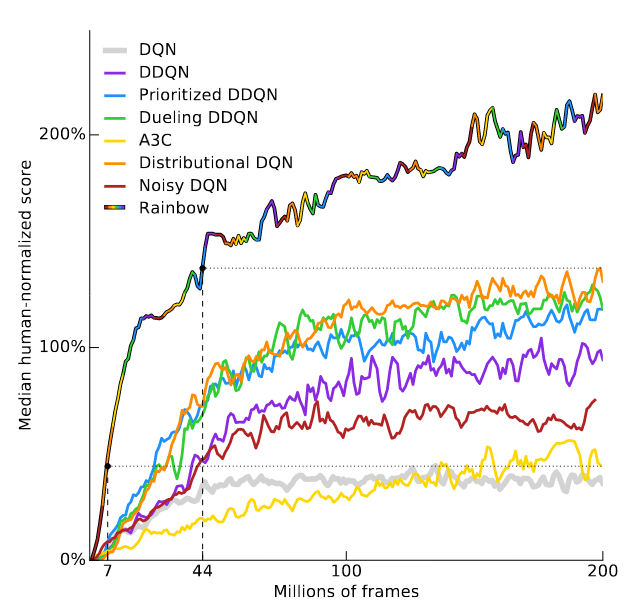
\includegraphics[scale=0.4]{neuralnetperformance}
        \label{fig:neuralnetperformance}
    \end{figure}

    When trying to create an agent that plays the online game Dota 2, \citet{berner19} used a Long Short-term Memory network.

    LSTMs\footnote{Long short-term memory network, type of ``recurrent neural network'' used in the field of deep learning capable of holding long-term dependencies.} were first defined by~\citet{hochreiter97} and improved upon in later works.
    An LSTM is an extension of the ``recurrent'' neural network, where nodes use feedback connections to allow the network to ``remember'' information in the long term.
    This solves the problem that traditional neural networks have, where they can't store information that can be useful to them in the long term.

    \subsection{Exploring Rogue}\label{subsec:exploring-rogue}
    The first notable instance of a program being developed to play Rogue was by~\citet{mauldin83}, where they created ``ROG-O-MATIC'', an expert system that plays Rogue.
    An expert system, as stated by~\citet{jackson86} in their book's introduction, ``is a computing system capable of representing and reasoning about some knowledge-rich domain''.
    Essentially, these systems aim to emulate a human expert in a particular domain and their decision-making.
    While expert systems are artificial intelligence, they make no use of machine learning to learn and adapt to situations, they follow what instructions have been programmed within them and are designed to rigidly solve one problem domain.

    An interface for machine learning agents to play Rogue has been created, called Rogueinabox~\citep{asperti17}.
    Rogueinabox is a framework that allow developers to create agents that interface with the game Rogue.
    In the Rogueinabox article, the authors ran a Deep Q-learning agent on the game for testing.
    They simplified the problem domain to have the agent only consider exploring the dungeon to find the stairs, without fighting or collecting items.
    Their agent performed reasonably well accounting dungeon exploration alone, however, the aim of our agent is to reach the Amulet of Yendor in the final floor.

    The initial agent proposed in the original Rogueinabox paper was further improved upon~\citep{asperti18}.
    The problem domain was still simplified to only consider getting to the exit stairs alone.
    While the previous implementation employed a DQN, the agent in the improvement implemented an A3C~\citep{mnih15}\footnote{Asynchronous Advantage Actor Critic, an asynchronous algorithm that aims to optimise a policy and estimate a value function by training multiple actors in parallel.} algorithm as a base, rather than a DQN. The A3C algorithm in the improvement was partitioned, meaning the sample space is \emph{partitioned} into a set of situations.
    This allows the different agents that run simultaneously to learn from different situations to build a common cumulative reward.
    It also involves the work by~\citet{jaderberg16}.

    Another interface that has been created is Rogue-gym~\citep{kanagawa19}.
    Rogue-gym is a game that accurately replicates the gameplay of Rogue while also allowing customisation of the game.
    It also comes with a customised OpenAI Gym environment which allows AI agents written in Python to interact with the game.
    The paper also shows an agent that was trained on a Proximal policy optimisation algorithm~\citep{schulman17}.

    \subsection{Exploring Other Roguelikes}\label{subsec:exploring-other-roguelikes}
    Rogue is not the only roguelike that has been explored with machine learning.
    NetHack, a popular roguelike game created in 1987, has been explored with machine learning during the development of the NetHack Learning Environment~\citep{kuttler20}.
    It is an environment that allows reinforcement learning agents to interact with NetHack easily.
    The paper introduces a baseline model that they trained on the environment.
    The map and player status are processed separately, concatenated, and run through an LSTM and a regular layer to produce the policy.

    An article by~\citet{izumiya21} explores how to involve the item inventory in the neural network system of a deep reinforcement learning agent with an attention-based approach.
    It is attention based as the system calculates a score for each item in an inventory using an ``attention function''.

    \section{Design and Methodology}\label{sec:design-and-methodology}
    \subsection{Problem Simplification}\label{subsec:problem-simplification}
    Due to the complex nature of the game, we introduce some simplifications to the problem so that
    we may create more manageable solutions.

    \begin{itemize}
        \item Monsters are disabled, so that combat is not part of the problem.
        \item The amount of actions available to the agent is reduced to the movement actions, search and wait.
        \item Initially we disabled hunger, so that the agent only needs to focus on descending the dungeon.
    \end{itemize}

    The objective of the neural network for chizuru-rogue is to take in the observed dungeon state as inputs and return an action that will maximise the expected reward as output as if it were maximising an action-value function.

    \subsection{Player Action}\label{subsec:action}
    Every action in Rogue is available to the player from the start of the game.

    When the player uses an action that utilises an item, the game will await the player to input a key.
    Every item in the player's inventory maps to one key on the keyboard.
    The player may input \texttt{*} to see what legal items they may choose and their corresponding key.
    Additionally, the player may see what the item-key mapping is by viewing their inventory with the \texttt{i} key at any time.

    \subsection{Neural Network}\label{subsec:neural-network}
    % TODO How are you going to compare Dueling DQN and Rainbow DQN? Is there a metric or multiple metrics? The tradeoff between metrics? Are they standard or ad hoc?
    The agent in our experiments will first utilise a base Dueling DQN, which will then be extended with Prioritised Experience Replay and finally extended with Noisy Networks and Multi-step Learning.
    Should time allow we will also introduce Distributional RL in order to create a full Rainbow DQN algorithm.

    % TODO write about the benefits and drawbacks of both dueling and rainbow

    \subsection{Agent Implementation}\label{subsec:implementation}
    The agent will be implemented in Python, which is one of the most popular languages used to model neural networks due to its many AI-related libraries that are available, including TensorFlow, which is what we use.
    TensorFlow provides tools for working with linear algebra and is widely used in machine learning.
    We chose TensorFlow over other alternatives such as PyTorch because it is one of the most popular frameworks for research,
    and it is bundled with Keras, a library that streamlines the creation and running of neural networks by providing the programmer with
    easy-to-use tools for defining, tuning and training neural network models.

    The agent will use Rogue-gym~\citep{kanagawa19} as an environment to interact with.
    
    \subsection{Experiments}\label{subsec:experiments} % TODO experiment discussion


    \subsection{Summary}\label{subsec:summary2}
    In this section we have outlined the algorithms and techniques we will use to create our agent, what we will use to implement them and how we will conduct our experiments.
    We have outlined our reasoning as to why we will use a Deep Q-network, mainly because it is a well-known algorithm that is proven to work well on a variety of game environments.
    The algorithms we will use are improvements to the base Deep Q-network algorithm: Dueling DQN, DDQN with Prioritised Experience Replay and DDQN with PER and Noisy Networks.
    If time allows, we will implement Distributional RL to introduce a full Rainbow DQN to the environment.
    We will compare these algorithms to see how they do when learning Rogue.

    \section{Agent Training and Results}\label{sec:agent-training-and-results}
    The agent was trained and evaluated on an Nvidia GeForce RTX 2080 graphics card using CUDA.

    Our training code was adapted from the work of~\citet{sebtheiler}.

    During our training of the agent, we measured the agent's performance with the following criteria after every run:

    \begin{itemize}
        \item The final score the agent achieved per episode (total reward)
        \item The deepest dungeon level the agent entered
    \end{itemize}

    \subsection{Dueling DQN}\label{subsec:dueling-dqn}
    In our first experiment, we ran our Dueling DQN for 13000 steps.
    From the results that can be seen in Figure~\ref{fig:ddqn_interval_score}, we were unable to extract a satisfactory result.
    Our model's average reward per interval\footnote{One interval is 10000 steps.} stagnated around 0.02, without increasing except one outlier of Interval 3, with an average reward of 0.049.
    Since the model could not increase its average reward, we set out to improve our model by configuring our hyperparameters and integrating Prioritised Experience Replay~\citet{schaul16} into our Dueling DQN for our second experiment.
    \begin{figure}[h]
        \caption[DDQN: Average reward per interval.]{Average reward per interval. One interval is 10000 steps.}
        \centering
        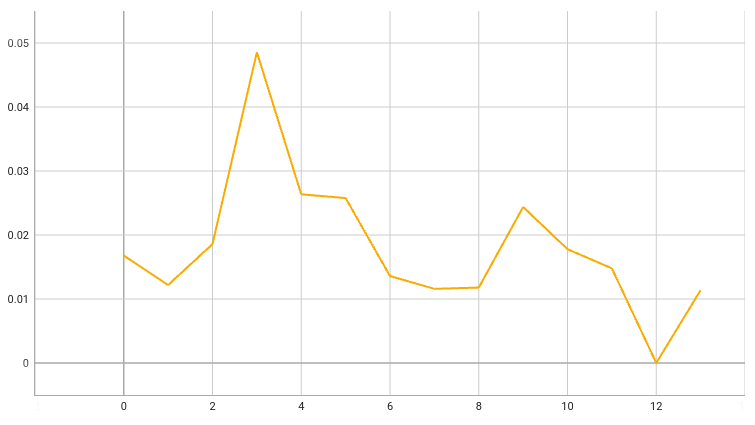
\includegraphics[scale=0.5]{interval_score_ddqn}
        \label{fig:ddqn_interval_score}
    \end{figure}

    \subsection{Dueling DQN with Prioritised Experience Replay}\label{subsec:dueling-dqn-with-prioritised-experience-replay}
    In our second experiment, we integrated Prioritised Experience Replay, another improvement to the DQN algorithm.
    As shown in Figure~\ref{fig:ddqn_per_interval_score}, we were also unable to extract a satisfactory result, with the average reward per interval stagnating over the entire training period.

    \begin{figure}[h]
        \caption[DDQN with PER: Average reward per interval.]{Average reward per interval. One interval is 10000 steps.}
        \centering
        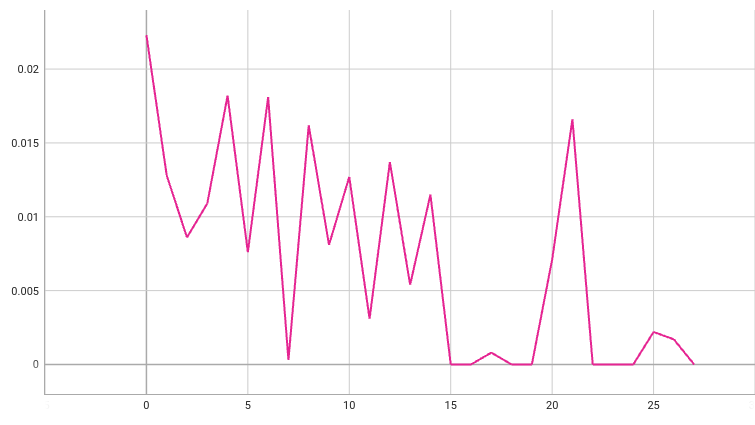
\includegraphics[scale=0.5]{interval_score_ddqn_per}
        \label{fig:ddqn_per_interval_score}
    \end{figure}



    \subsection{Dueling DQN with Prioritised Experience Replay, Noisy Networks and Multi-step Learning}\label{subsec:dueling-dqn-with-prioritised-experience-replay-and-noisy-networks}
    \textbf{Need to be added.}

    \section{Conclusion}\label{sec:conclusion}
    In this paper we have set out to improve upon to~\citet{asperti18} and ~\citet{kanagawa19}`s tests by utilising extensions to the DQN algorithm
    to perform dungeon crawling in Rogue's randomly generated dungeons, testing a combination of multiple improvements in order to
    provide a perspective on the performance.

    We have achieved the following in this article:
    \begin{itemize}
        \item Implementation of a Dueling DQN as well as two different improvements for learning the game Rogue
        \item Deployment of our neural network to run experiments
    \end{itemize}

    % TODO go into detail about the actual achievements

    However, our goal was to achieve a successful improvement upon previous literature, but our models did not achieve satisfactory results.
    The average reward per interval that our models attained did not increase as the model learnt.
    This could be due to either more training being required, or our model needing improvement, as we describe in depth in Section~\ref{subsec:future-work}.

    Our main challenge was creation of the neural network.


    Another challenge we faced was tuning of hyperparameters.
    We experimented with several configurations of hyperparameters, and the hyperparameters we used for our tests are noted in Section~\ref{subsec:hyperparameters}.
    Since we were unsuccessful in obtaining satisfactory results, we must improve upon how we tune our hyperparameters as described in Section~\ref{subsec:future-work}.

    Our work provides a framework to...

    This project was good to develop...

    % Explain where chizuru performed well, where it screwed up, and the most important aspect about it

    % Talk about the neural network here
    
    \subsection{Future work}\label{subsec:future-work}
    As we were unsuccessful in achieving a satisfactory result, the future work for this project aims to rectify this.
    Looking at what we have accomplished and read, we have identified four main areas of improvement for future work.

    The first is memory management of our program.
    During training of our agent, we ran into an issue where our program was gradually using up more and more memory on the system.
    This means that training of our agent would have to be interrupted periodically so that it would not impact other processes on the system, decreasing the efficiency of training.
    We ran the Fil memory profiler\footnote{\url{https://pythonspeed.com/fil/}} on our program and discovered that predicting an action to take for our agent was taking up the bulk of memory as can be seen in Figure~\ref{fig:fil}.
    In future work investigation into why these memory issues occur should be performed and how to mitigate them.

    \begin{figure}[h]
        \caption[Fil Profiler result for DDQN with PER.]{Fil memory profiler result for our DDQN with PER. Larger bars with a deeper shade of red means the line took up more memory.}
        \centering
        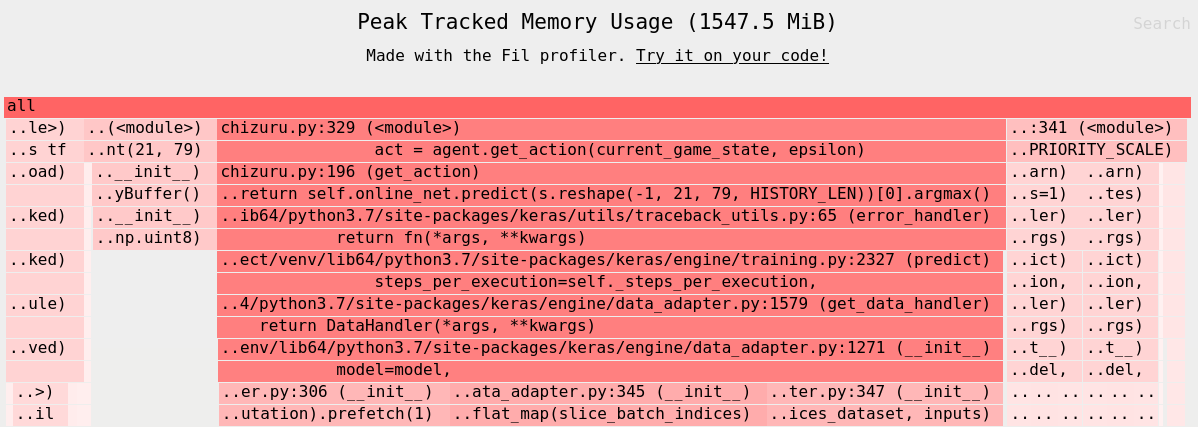
\includegraphics[scale=0.3]{fil}
        \label{fig:fil}
    \end{figure}

    Secondly is the reward function.
    The reward function currently provides a reward of 0 for moving in the map without collecting gold or descending stairs.
    In

    Network architecture

    The fourth is hyperparameter tweaking.
    As we did not obtain satisfactory results for our neural network, in future work more research on what hyperparameters
    are used in what configuration of neural networks and environments are used should be conducted.
    In addition, more experiments on how different configurations of hyperparameters should also be performed.

    \subsection{Reflection}\label{subsec:reflection}

    % Write some bollocks on how RL works well on video games and how this can lead to real-world developments with this technology. End off on a positive note!


    %%%%% Everything after here is not counted in the word count. %%%%%
    \medskip

    \bibliographystyle{agsm}
    \bibliography{diss}

    \medskip

    \appendix
    \section*{Appendices}
    \addcontentsline{toc}{section}{Appendices}
    \section{Methods}\label{sec:methods}

    \subsection{State Representation}\label{subsec:state-representation}
    The state of the game is converted from a 21x79 grid of ASCII characters as displayed to a human player to a 21x79 grid of
    numbers each representing one character using rogue-gym's \texttt{state.gray\_image()} function.

    \subsection{Reward Representation}\label{subsec:reward-representation}
    The reward signals are as follows
    \begin{itemize}
        \item Reward per movement: 0
        \item Reward for collecting gold: based on gold collected
        \item Reward for descending stairs: 100
    \end{itemize}

    \subsection{Hyperparameters}\label{subsec:hyperparameters}
    \subsubsection{Dueling DQN - First Run}
    \begin{lstlisting}[label={lst:ddqn1hyperparameters}]
GAMMA = 0.99
NUM_ITERATIONS = 20000
MAX_TURNS_IN_EPISODE = 1000
BATCH_SIZE = 32
BUFFER_SIZE = 200000
MIN_REPLAY_SIZE = 400
EPSILON_START = 1.0
EPSILON_END = 0.01
EPSILON_DECAY = 150000
LEARNING_RATE = 0.00001
LEARNING_FREQUENCY = 1000
TARGET_UPDATE_FREQUENCY = 1000
    \end{lstlisting}

    \subsubsection{Dueling DQN - Second Run}
    \begin{lstlisting}[label={lst:ddqn2hyperparameters}]
GAMMA = 0.99
NUM_ITERATIONS = 20000
MAX_TURNS_IN_EPISODE = 1250
BATCH_SIZE = 32
BUFFER_SIZE = 200000
MIN_REPLAY_SIZE = 1500
EPSILON_START = 1.0
EPSILON_END = 0.01
EPSILON_DECAY = 150000
LEARNING_RATE = 0.00001
LEARNING_FREQUENCY = 75
TARGET_UPDATE_FREQUENCY = 750
    \end{lstlisting}

    \subsubsection{Dueling DQN/Prioritised Experience Replay}
    \begin{lstlisting}[label={lst:ddqnperhyperparameters}]
GAMMA = 0.99
NUM_ITERATIONS = 20000
MAX_TURNS_IN_EPISODE = 1250
BATCH_SIZE = 32
BUFFER_SIZE = 100000
MIN_REPLAY_SIZE = 1500
EPSILON_START = 1.0
EPSILON_END = 0.01
EPSILON_DECAY = 150000
LEARNING_RATE = 0.00001
LEARNING_FREQUENCY = 75
TARGET_UPDATE_FREQUENCY = 750
PRIORITY_SCALE = 0.7
    \end{lstlisting}

    \subsubsection{Dueling DQN/Noisy Networks}

    \subsection{Network Architecture}\label{subsec:network-architecture}
    \subsubsection{Dueling DQN}
    \begin{lstlisting}[label={lst:dueling}]
    net_input = tf.keras.Input(shape=(h, w, 4))
    net_input = tf.keras.layers.Lambda(lambda layer: layer / 255)(net_input)

    conv1 = tf.keras.layers.Conv2D(32, (3, 3), strides=2, activation="relu")(net_input)
    conv2 = tf.keras.layers.Conv2D(64, (3, 3), strides=1, activation="relu")(conv1)
    conv3 = tf.keras.layers.Conv2D(64, (3, 3), strides=1, activation="relu")(conv2)

    val, adv = tf.keras.layers.Lambda(lambda ww: tf.split(ww, 2, 3))(conv3)

    val = tf.keras.layers.Flatten()(val)
    val = tf.keras.layers.Dense(1)(val)

    adv = tf.keras.layers.Flatten()(adv)
    adv = tf.keras.layers.Dense(len(ACTIONS))(adv)

    reduced = tf.keras.layers.Lambda(lambda ww: tf.reduce_mean(ww, axis=1, keepdims=True))

    output = tf.keras.layers.Add()([val, tf.keras.layers.Subtract()([adv, reduced(adv)])])

    final_model = tf.keras.Model(net_input, output)

    final_model.compile(
        optimizer=tf.keras.optimizers.Adam(learning_rate=LEARNING_RATE),
        loss=tf.keras.losses.MeanSquaredError(),
        metrics=[tf.keras.metrics.SparseCategoricalAccuracy()]
    )

    return final_model
    \end{lstlisting}

    \subsubsection{Dueling DQN/Noisy Networks}


\end{document}
